\documentclass[twoside,twocolumn]{article}
\usepackage{blindtext}
\usepackage{graphicx}
\usepackage[sc]{mathpazo}
\usepackage[T1]{fontenc}
\linespread{1.05}
\usepackage{microtype}
\usepackage[english]{babel}
\usepackage[hmarginratio=1:1,top=32mm,columnsep=20pt]{geometry}
\usepackage[hang, small,labelfont=bf,up,textfont=it,up]{caption}
\usepackage{booktabs}
\usepackage{lettrine}
\usepackage{enumitem}
\setlist[itemize]{noitemsep}
\usepackage{abstract}
\renewcommand{\abstractnamefont}{\normalfont\bfseries}
\renewcommand{\abstracttextfont}{\normalfont\small\itshape}
\usepackage{titlesec}
\renewcommand\thesection{\Roman{section}}
\renewcommand\thesubsection{\roman{subsection}}
\titleformat{\section}[block]{\large\scshape\centering}{\thesection.}{1em}{}
\titleformat{\subsection}[block]{\large}{\thesubsection.}{1em}{} 
\usepackage{fancyhdr}
\fancyhead{}
\fancyfoot{}
\fancyfoot[RO,LE]{\thepage}
\usepackage{titling}
\usepackage{hyperref}
\setlength{\droptitle}{-4\baselineskip} 
\pretitle{\begin{center}\Huge\bfseries}
\posttitle{\end{center}}
\title{Sudoku solver}
\author{
\textsc{Gaetano Conti, Vincenzo Imperati}\\[1ex]
}
\date{14 Gennaio 2021}
\renewcommand{\maketitlehookd}{
	\begin{abstract}
	\noindent
	Questo documento presenta un approccio multithreading alla risoluzione di sudoku 9x9 mediante le librerie Pthread e OpenMP. Vengono discusse due soluzioni, una per ogni libreria adottata. La soluzione che adotta Pthread, svolge una ricerca in profondità in parallelo su più thread. La soluzione che adotta OpenMP svolge una ricerca in ampiezza parallelizzando alcune parti del codice là dove possibile. Nel documento vengono descritte le architetture delle due soluzioni, i problemi riscontrati, le limitazioni ed in fine vengono riportati i test svolti su di un dataset comune di sudoku 9x9. Le due soluzioni multithreading proposte vengono comparate tra loro ed infine vengono comparate con la loro versione sequenziale. Il dataset è composto da soli sudoku con un'unica soluzione. 
	\end{abstract}
}
\begin{document}
\maketitle
\section{Sudoku solver Pthread}
La seguente soluzione è derivata da una visita ricorsiva in profondità (DFS). La DFS permette di visitare l'intero albero delle possibili soluzioni del sudoku dato da risolvere. Questo tipo di approccio è vantaggioso qualora la soluzione si trovasse in profondità, invece che in superficie (dove performa meglio la BFS).

Questa soluzione svolge una visita DFS sull'albero delle possibili soluzioni del sudoku dato in input, utilizzando un numero di thread dato in input. Lo scopo è trovare l'unica soluzione del sudoku svolgendo la DFS in modo parallelo sfruttando la potenza computazionale di più thread. L'obiettivo è anche riuscire a distribuire in modo ottimale il lavoro computazionale che ogni thread deve svolgere.

L'algoritmo acquisisce in input il numero di thread che è chiamato ad utilizzare, e acquisisce il sudoku da validare (trovare l'univoca soluzione). Durante l'acquisizione del sudoku viene riempita la griglia di 81 celle e vengono memorizzate in una lista le coordinate delle celle vuote. Questa lista ha lo scopo di identificare le celle vuote senza il bisogno di leggere la griglia. In questa lista le celle vuote vengono memorizzate in ordine di lettura e vengono lette nel verso opposto qualora un thread dovesse interrogare la lista delle celle vuote per provare a riempirne una.

{\itshape Durante l'ottimizzazione dell'algoritmo si è pensato di mescolare l'ordine delle celle vuote nella lista con l'intuizione di risolvere in minor tempo il sudoku con il beneficio del fatto che si sarebbero riempite le celle in modo sparso e non in modo lineare. Quest'intuizione si è rivelata sbagliata siccome nella pratica è risultato più efficiente risolvere il sudoku riempiendo in modo lineare le celle vuote del sudoku.}

Una volta terminata l'acquisizione dell'input, l'algoritmo ha tutto ciò di cui ha bisogno per validare il sudoku. A questo punto vengono inizializzate le variabili utili per una corretta cooperazione tra thread. Di seguito vengono quindi descritte le variabili principali per poter comprendere al meglio l'algoritmo.

\begin{description}
	\addtolength{\itemindent}{0.5cm}
	\itemsep0em
	\item [problem\_solved] intero che se diverso da zero indica che un sudoku valido è stato trovato.
	\item [sudokus\_to\_solve] lista di sudoku da validare, uno per ogni thread. L'Idle Validator thread, prende da qui il sudoku da validare.
	\item [semaphores] lista di semafori, uno per ogni thread. Gli Idle Validator threads attendono sul proprio semaforo in attesa di diventare Active Validator threads. Saranno i Delegator threads a svegiare gli Idle Validator threads.
	\item [mutex\_shared\_data] mutex per accedere in mutua esclusione alla FIFO.
	\item [shared\_fifo\_idle\_threads] FIFO condivisa tra i vari thread.
	\item [mutex\_solved\_sudoku] mutex per accedere in mutua esclusione alla scrittura del sudoku che conterrà una grid valida.
	\item [solved\_sudoku] sudoku che conterrà una grid valida.
\end{description}

Di seguito viene riportata una descrizione dei possibili stati di un thread per comprendere meglio le varie funzioni che un thread è chiamato a svolgere.

\begin{description}
	\addtolength{\itemindent}{0.5cm}
	\itemsep0em
	\item [Idle Validator] Il thread in questo stato e inattivo, quindi non sta validando nessun sudoku. Esso è visibile nella FIFO dai Delegator thread ed è quindi in attesa di un sudoku da validare.
	\item [Active Validator] Il thread in questo stato è attivo, quindi sta validando il sudoku che gli è stato assegnato.
	\item [Delegator] Il thread in questo stato è attivo, svolge lo stesso compito di un qualsiasi Active Validator. La differenza è che un Delegator ha la possibilità di delegare ad un Idle Validator una parte di computazione che deve svolgere per validare il sudoku che gli è stato assegnato da validare.
\end{description}
			
\begin{figure}[htp]
\begin{center}
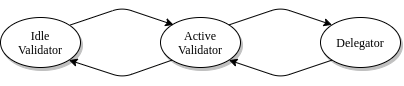
\includegraphics[width=0.45 \textwidth]{stati thread.png}
\caption{Possibili stati dei thread}
\end{center}
\end{figure}

A questo punto L'algoritmo lancia i thread che inizialmente sono tutti Idle Validator, quindi verrà assegnato ad un thread il sudoku acquisito in input come sudoku da validare. Così facendo questo thread è il primo a diventare Active Validator e procede con la validazione del sudoku assegnatogli. 

La validazione consiste nel riempire le celle vuote nel modo corretto, però per riempire una cella vi possono essere più possibilità, ovvero più numeri sono validi per una cella vuota. Quindi occorre percorrere tutte queste possibilità, e l'unico modo è quello di validare non più un solo sudoku, ma validare tutti i sudoku che vengono generati dalla possibilità di riempire una cella vuota con tutti i numeri validi per quella cella.
\\\indent
Il singolo thread quindi si ritrova a dover validare un gruppo di sudoku, così prima di intraprendere qualsiasi validazione controlla se c'è un Idle Validator che attende un sudoku da validare. Nel caso questo fosse disponibile, il thread che possiede i sudoku da validare diventa Delegator e delega la validazione di un sudoku al primo Idle Validator in attesa.
\\\indent
In questo modo tutti gli Active Validators cercano di diventare Delegators per poter delegare i sudoku che hanno da validare, cedendoli così ai primi Idle Validators in attesa. Così facendo tutta la computazione viene equamente distribiuta tra i thread, perchè qualora ci fosse un Idle Validator in attesa di sudoku da validare, ci sarà sempre un Active Validator che prova a divetare Delegator per delegare un sudoku ancora da validare, oppure un Delegator che già lo sta facendo.
\\\indent
{\itshape Nell'algoritmo presentato i Delegator possono delegare solo un sudoku alla volta, quindi possono attivare un solo Idle Validator alla volta. Questo comunque non penalizza assolutamente l'efficiente distribuzione di computazione tra i thread, perchè questa è già intrinsecamente bilanciata dall'architettura dell'algoritmo. Ciò non toglie che un Delegator possa delegare tutti i sudoku ancora da validare, fino ad esaurimento dei sudoku in suo possesso o esaurimento di Idle Validator. Questa variante si avvicina di più ad una logica BFS, ovvero più sudoku deleghiamo nello stesso momento più thread valideranno sudoku posti allo stesso livello. Alla luce di questa possibilitstatà è stata programmata anche una versione dell'algoritmo che permette di decidere il numero massimo di sudoku da poter delegare in una sola volta potendo così decidere quanto rendere l'algoritmo più propenso ad una visita in ampiezza rispetto ad una visita in profondità. In questo modo è possibile modulare la tipologia di visita per ottimizzare al meglio la risoluzione di un sudoku. Siccome i sudoku sono sempre diversi è diveso quindi il punto nell'albero in cui è situata la soluzione al sudoku. Questa variante non è stata presentata come algoritmo principale perchè non è stata coperta una criticità nell'algoritmo che salta fuori con un determinato schedule dei thread una volta trovata la soluzione. Questa variante è comunque valida ma a causa di questa criticità (che non è stata risolta per problemi di tempo) non è stata adoperata durante i test.}
\\\indent
L'algoritmo termina quando un Active Validator riesce a riempire l'ultima cella vuota di un sudoku che gli è dato da validare con un numero valido. A questo punto copia questo sudoku in solved\_sudoku e notifica tramite problem\_solved che è stato trovato un sudoku valido. Così facendo gli altri thread terminano di conseguenza.


\section{Sudoku solver OpenMP}
La seguente soluzione è derivata da una visita in ampiezza (BFS). La BFS permette di visitare l'intero albero delle possibili soluzioni del sudoku dato da risolvere. Questo tipo di approccio è vantaggioso qualora la soluzione si trovasse in superficie, invece che in profondità (dove performa meglio la DFS).

Questa soluzione svolge una visita BFS sull'albero delle possibili soluzioni del sudoku dato in input, utilizzando un numero di thread dato in input. Lo scopo è trovare l'unica soluzione del sudoku svolgendo la BFS in modo parallelo sfruttando la potenza computazionale di più thread. L'obiettivo è anche riuscire a distribuire in modo ottimale il lavoro computazionale che ogni thread deve svolgere.

L'algoritmo acquisisce in input il numero di thread che è chiamato ad utilizzare, e acquisisce il sudoku da validare (trovare l'univoca soluzione). Durante l'acquisizione del sudoku viene riempita la griglia di 81 celle e vengono memorizzate in una lista le coordinate delle celle vuote. Questa lista ha lo scopo di identificare le celle vuote senza il bisogno di leggere la griglia. In questa lista le celle vuote vengono memorizzate in ordine di lettura e vengono lette nel verso opposto qualora un thread dovesse interrogare la lista delle celle vuote per provare a riempirne una.

{\itshape Durante l'ottimizzazione dell'algoritmo si è pensato di mescolare l'ordine delle celle vuote nella lista con l'intuizione di risolvere in minor tempo il sudoku con il beneficio del fatto che si sarebbero riempite le celle in modo sparso e non in modo lineare. Quest'intuizione si è rivelata sbagliata siccome nella pratica è risultato più efficiente risolvere il sudoku riempiendo in modo lineare le celle vuote del sudoku.}

Una volta terminata l'acquisizione dell'input, l'algoritmo ha tutto ciò di cui ha bisogno per validare il sudoku. A questo punto vengono inizializzate le variabili utili per una corretta cooperazione tra thread. Di seguito vengono quindi descritte le variabili principali per poter comprendere al meglio l'algoritmo.

\begin{description}
	\addtolength{\itemindent}{0.5cm}
	\itemsep0em
	\item [solved\_sudoku] intero che se diverso da zero indica che un sudoku valido è stato trovato.
    \item [list] lista contenente tutti i sudoku da validare. Inizialmente contiene solo il sudoku acquisito in input.
    \item [index\_list] indice di list, ci permette di operare sulla list.
    \item [new\_list] lista contenente il nuovo livello di sudoku da validare. Questa lista si ottiene da tutti i possibili sudoku che vengono generati quando si cerca di riempire una cella vuota di ogni sudoku in list, generando in alcuni casi nuovi sudoku da dover validare. Così facendo i nuovi sudoku da validare sono quelli in nex\_list.
    \item [new\_index\_list] indice di new\_list, ci permette di operare sulla new\_list.
\end{description}

A questo punto l'algoritmo procede con una BFS che consiste nel visitare il livello successivo dell'albero creando la new\_list tramite l'ultimo livello visitato rappresentato da list. La new\_list viene riempita di sudoku da validare inseriti dai thread che parallelizzano questo inserimento. L'inserimento in new\_list di questi sudoku deve avvenire necessariamente in modo sequenziale, ma tutte le computazioni di contorno possono avvenire in parallelo. Infatti i thread sono chiamati a parallelizzare il doppio ciclo di for che permette la compilazione di new\_list. 
\\\indent
Una volta che un thread riesce a riempire l'ultima cella vuota di un sudoku notifica tramite solved\_sudoku che è stato trovato un sudoku valido e scrive questo sudoku nella memoria occupata dal sudoku che rappresenta la soluzione, così alla fine della compilazione di new\_list l'algoritmo può terminare.
\\\indent
{\itshape Si noti che tramite questa risoluzione si ha un elevato dispendio di memoria se la soluzione si dovesse trovare in profondità, questo quindi comporterebbe allocare molta memoria per memorizzare tutti i sudoku presenti in un livello molto profondo dell'albero.}

\section{Test e risultati} 	%à, è, ì, ò, ù,
Le due soluzioni proposte sono state testate su uno stesso dataset di 100 sudoku. I test sono stati effetuati su una macchina con una CPU Intel(R) Core(TM) i7-6500U e una RAM di 8 GB. Ogni soluzione è stata eseguita con le seguenti quantità di thread a disposizione: 1, 2, 4, 8, 16, 32. Di seguito sono riportati due grafici per ognuna delle due soluzioni descritte. 
\\\indent
{\itshape Si noti che il dataset è ponderato sulle prestazioni della soluzione che adotta OpenMP, siccome è la soluzione meno efficente per velocità di risoluzione e uso della memoria.}

\subsection{Pthread}
Il primo grafico mostra le prestazioni dell'algoritmo eseguito con le quantità di thread a disposizione. Si noti che l'esecuzione con due thread ha una prestazione migliore che con uno solo. All'aumentare del numero dei thread le prestazioni si vanno a deteriorare. 
\\\indent Il secondo grafico mette in confronto le prestazioni dell'algoritmo eseguito con un solo thread con le migliori prestazioni ottenute dalle versioni multi-thread alla luce dello stesso sudoku. Si noti che vi è una netta differenza prestazionale.

\begin{figure}[htp]
\begin{center}
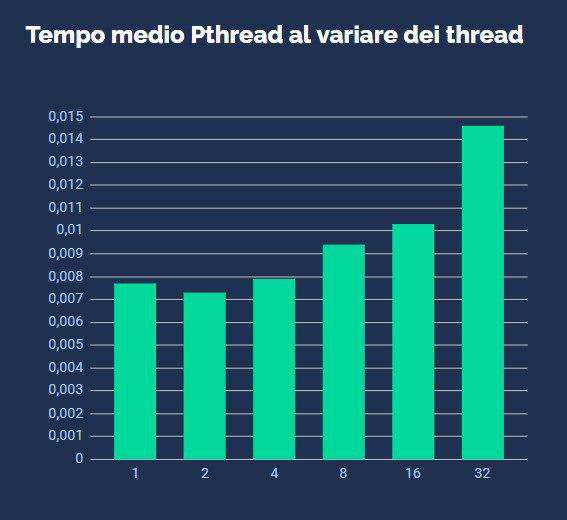
\includegraphics[width=0.4 \textwidth]{Test Pthread.png}
\caption{Test Pthread}
\end{center}
\end{figure}

\begin{figure}[htp]
\begin{center}
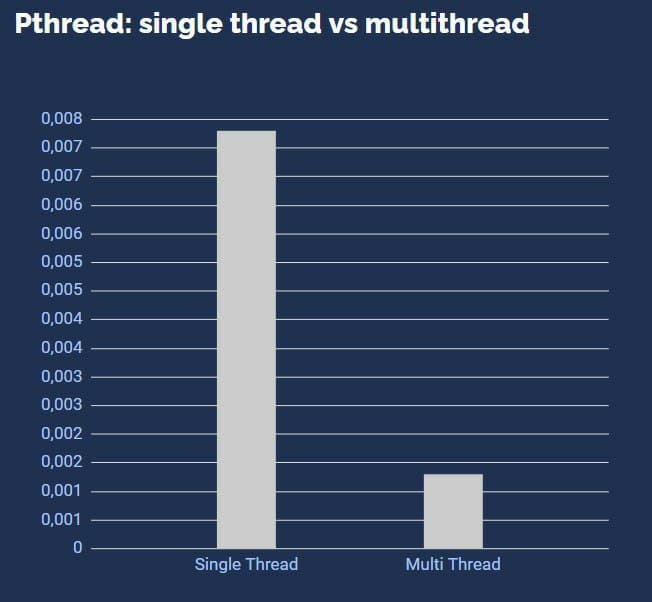
\includegraphics[width=0.4 \textwidth]{Pthread single vs multi.png}
\caption{Single-core vs Multi-core - Pthread}
\end{center}
\end{figure}

\subsection{OpenMP}
Il primo grafico mostra le prestazioni dell'algoritmo eseguito con le quantità di thread a disposizione. Si noti che non vi è un netto miglioramento prestazionale attraverso l'utilizzo di più thread.
\\\indent Il secondo grafico mette in confronto le prestazioni dell'algoritmo eseguito con un solo thread con le migliori prestazioni ottenute dalle versioni multi-thread alla luce dello stesso sudoku. Si noti che la soluzione multithreading proposta non performa meglio di quella sequenziale.

\begin{figure}
\begin{center}
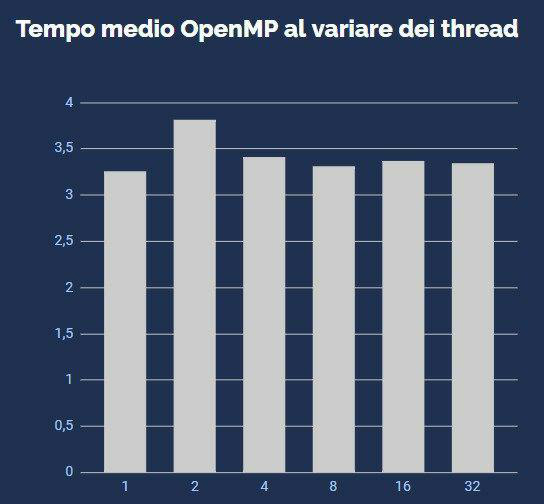
\includegraphics[width=0.4 \textwidth]{Test OpenMP.png}
\caption{Test OpenMP}
\end{center}
\end{figure}

\begin{figure}
\begin{center}
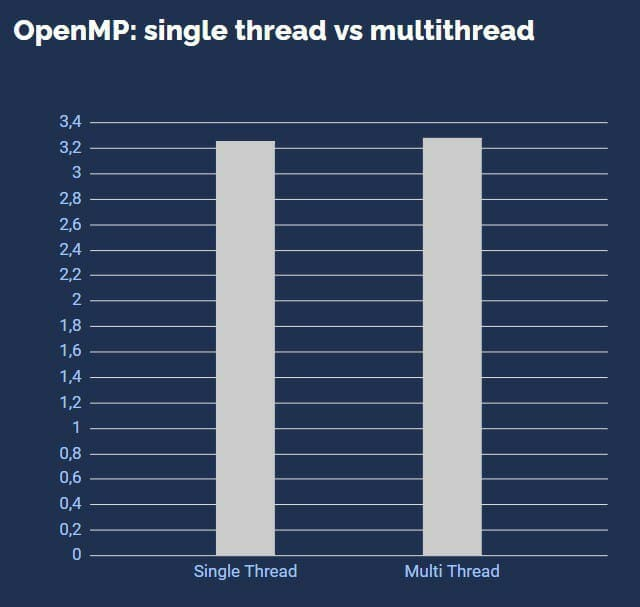
\includegraphics[width=0.4 \textwidth]{OpenMP single vs multi.png}
\caption{Single-core vs Multi-core - OpenMP}
\end{center}
\end{figure}

\end{document}
